\chapter{Modelo e implementación}
\pagenumbering{arabic}
Para la realización de este trabajo, se han diseñado y desarrollado una serie de agentes a los que se les ha entrenado para la obtención de un comportamiento de fototaxis, es decir, de
búsqueda y acercamiento a fuentes de luz.

Cada agente esta modelado como un círculo con dos sensores en la parte frontal y dos motores opuestos que permiten que el agente pueda moverse libremente por el espacio, como puede verse
en la figura XXXXXX. El agente tiene en todo momento una posición en el espacio dada por unas coordenadas (x, y), así como una orientación respecto al eje X. Cada sensor esta separado
60º del eje de orientación del agente.

\begin{figure}[!h]
	\centering
	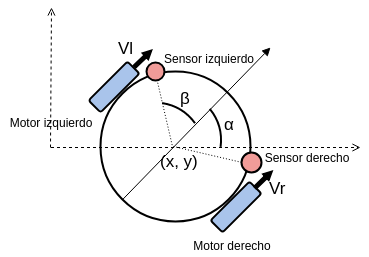
\includegraphics[width=0.8\textwidth,height=6cm]{Imagenes/Agent}
	\caption{Esquema del agente utilizado.}
	\label{fig:figuraMyAgent}
\end{figure}

El movimiento traslacional del agente se calcula a partir de la velocidad lineal ($v$) de su centro de masa (XXXX formula). El movimiento angular del agente se calcula obteniendo
la velocidad angular ($\omega$) de su centro de masa (XXXXXX formula).

\begin{equation} \label{eq:VFormula}
 \centering
 v = \frac{Vr + Vl}{2}
\end{equation}

\begin{equation} \label{eq:WFormula}
 \centering
 \omega = \frac{Vr - Vl}{2R}
\end{equation}

La nueva posición del agente para cada ciclo de ejecución se calcula mediante las fórmulas (XXX formulaX formulaY formulaA), donde $x$ e $y$ representan la posición actual del agente,
$\theta$ representa la orientación actual del agente y $\delta t$ representa el tamaño del tiempo de integración de ciclo.

\begin{equation} \label{eq:newXformula}
 \centering
 x(t + 1) = x(t) + v.cos(\theta).\delta t
\end{equation}

\begin{equation} \label{eq:newYformula}
 \centering
 y(t + 1) = y(t) + v.sin(\theta).\delta t
\end{equation}

\begin{equation} \label{eq:newAformula}
 \centering
 \delta (t + 1) = \delta (t) + \omega .\delta t
\end{equation}

Para los experimentos realizados en este trabajo, el radio del agente siempre es \textbf{4.0}.

\subsection{Controlador}
Hablar de la red, numero de neuronas etc etc etc etc
\subsection{Plasticidad}
La ultraestabilidad del agente se ha conseguido dotando al mismo de mecanismos de plasticidad, que le permiten modificar los valores de algunos de sus atributos internos. En este caso, los agentes pueden
alterar los valores de los pesos $w_{ij}$ de las conexiones entre las neuronas de la red cuando la frecuencia de activación de una neurona es demasiado baja o demasiado alta.

La homeostasis no se encuentra programada explícitamente, pero aparece de forma implícita debido a los mecanismos de evaluación de la evolución genética que recompensan con mejor puntuación a aquellos
agentes que, durante la realización del entrenamiento, han mantenido un mayor número de sus neuronas estables.

La plasticidad de cada conexión esta gobernada por la actividad sináptica de la conexión junto con una regla de plasticidad codificada genéticamente. Estas reglas de plasticidad vienen dadas por las
ecuaciones (LISTA DE FORMULAS XXXX), donde $\Delta w_{ij}$ es el incremento por unidad de tiempo de un determinado peso sináptico ($w_{ij}$), y $z_{i}$ y $z_{j}$ son las frecuencias de
activación de las neuronas presinápticas y postsinápticas respectivamente.

Las reglas de plasticidad se construyen en torno a cuatro parámetros: la frecuencia de aprendizaje ($n_{ij}$), un valor límite ($z_{ij}^{o}$), el grado de facilitación plástica local ($p_{j}$) y
un factor de amortiguación linear que restringe el cambio dentro de los limites establecidos para los valores de los pesos sinápticos ($\delta$).

\noindent
R0: Sin plasticidad:
\begin{equation} \label{eq:R0plasticityRule}
 \centering
 \Delta w_{ij}= 0
\end{equation}
\noindent
R1: Aprendizaje Hebbiano acotado:
\begin{equation} \label{eq:R1plasticityRule}
 \centering
 \Delta w_{ij}= \delta n_{ij} p_{j} z_{i} z_{j}
\end{equation}
\noindent
R2: Potenciación o depresión amortiguadas de la neurona presináptica cuando la eficacia sináptica es muy alta o muy baja:
\begin{equation} \label{eq:R2plasticityRule}
 \centering
 \Delta w_{ij}= \delta n_{ij} p_{j} (z_{i} - z_{ij}^{o}) z_{j}
\end{equation}
\noindent
R3: Potenciación o depresión amortiguadas de la neurona postsináptica cuando la eficacia sináptica es muy alta o muy baja:
\begin{equation} \label{eq:R3plasticityRule}
 \centering
 \Delta w_{ij}= \delta n_{ij} p_{j} z_{i} (z_{j} - z_{ij}^{o})
\end{equation}

El grado de facilitación plástica local ($p_{j}$) se ve incrementado linealmente (hasta un valor máximo de 1) cuando la frecuencia de activación aumenta hasta salirse de sus límites, facilitando
así los cambios plásticos. Cuando la frecuencia de activación entra en sus límites, $p_{j}$ decrece linealmente (hasta un valor mínimo de -1), disminuyendo la facilidad de los cambios plásticos.

El cambio en la conexión sináptica depende del signo de $n_{ij}$, de forma que cada neurona puede actuar de manera independiente facilitando los cambios plásticos en la dirección indicada.

El factor de amortiguación lineal ($\delta$) asegura que los valores de los pesos se mantienen dentro de los límites establecidos para ellos.

El factor de valor límite ($z_{ij}^{o}$) depende linealmente del valor actual del peso que se está actualizando plásticamente, por lo que es calculado en cada modificación.

Los pesos son actualizados cada iteración (si precede, dependiendo de su regla de plasticidad) a partir de la ecuación ECUACION XXXX.
\begin{equation} \label{eq:WeightUpdate}
 \centering
 w_{ij}(t+1) = w_{ij}(t) + \Delta w_{ij}
\end{equation}



\section{Agente}
TODO: Hablar de la forma del agente y de las configuraciones elegidas en temas de rangos y plasticidades

\subsubsection{Estructura de la red, simetría y rangos de valores utilizados}
La CTRNN utilizada para la realización de este experimento esta compuesta por ocho neuronas totalmente interconectadas entre sí, presentando la estructura que puede observarse en la figura 3.2.
Las dos primeras neuronas (0 y 1 en la figura 3.2) serán las que se encuentren conectadas a los dos sensores y por tanto las que reciben sus mediciones y las procesen. Las dos últimas neuronas
(6 y 7 en la figura 3.2) serán las que se encuentren conectadas a los dos motores, los cuales procesarán las salidas de estas neuronas para calcular las velocidades de cada uno de ellos.

\begin{figure}[!h]
	\centering
	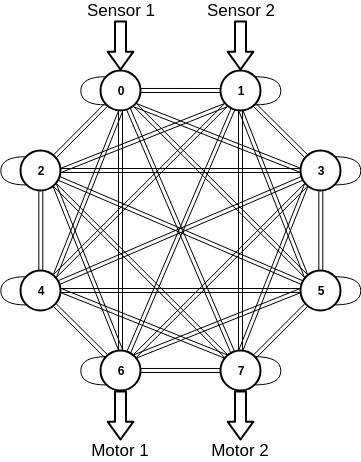
\includegraphics[width=0.4\textwidth,height=7cm]{Imagenes/MyRed}
	\caption{Esquema de la estructura de la red utilizada con 8 neuronas totalmente interconectadas.}
	\label{fig:figuraMyRed}
\end{figure}

\begin{table}[!h]
\centering
\label{table:tablaValoresParametros}
\begin{tabular}{l|l|c|c}
\textbf{Parametro} & \textbf{Descripción}          & \multicolumn{1}{l|}{\textbf{Valor mínimo}} & \multicolumn{1}{l}{\textbf{Valor máximo}} \\
\textit{$\tau_{i}$}       & Constante de decaimiento      & 0.4                                        & 4.0                                       \\
\textit{$\theta{i}$}      & Bias                          & -3.0                                       & 3.0                                       \\
\textit{Gain}      & Ganancia motora y sensora     & 0.1                                        & 10.0                                      \\
\textit{$w_{ij}$}      & Peso de la conexión sináptica & -10.0                                      & 10.0                                      \\
\textit{$n_{ij}$}     & Ritmo de plasticidad          & -0.9                                       & 0.9
\end{tabular}
\caption{Rango de valores para los parámetros de la red}
\end{table}

Para la realización de los experimentos se utilizarán CTRNNs en las que todas las neuronas
estén totalmente interconectadas (conexión de cada neurona con todas las demás en ambas direcciones) y
autoconectadas (conexión recurrente de la neurona a sí misma).

Como mínimo la CTRNN contará con cuatro neuronas. Dos de ellas conectadas cada una a uno de los dos sensores del agente y las otras dos conectadas cada una a uno de los dos motores del agente (además de
tener el resto de conexiones anteriormente descritas).

La red contará con una cierta simetría en las ganancias de las neuronas sensoras y motoras. Teniendo las dos neuronas conectadas a los sensores del agente iguales ganancias entre si, al igual que las dos neuronas conectadas
a los motores del agente.
